%%%%%%%%%%%%%%%%%%%%%%%%%%%%%%%%%%%%%%%%%%%%%%%%%%%%%%%%%%%%%%%%%%%%%%%%
%
% Template latex file for a common article class for class notes
% and write ups. Additional Configuration and styling options are 
% commented out. ex. Table of Contents and Title page
% 
% Author: Amy Bui
% 
%%%%%%%%%%%%%%%%%%%%%%%%%%%%%%%%%%%%%%%%%%%%%%%%%%%%%%%%%%%%%%%%%%%%%%%%
 
\documentclass[12pt]{article}
\usepackage[utf8]{inputenc}
\usepackage{parskip}
\usepackage{tabularx}
\usepackage{array}
\usepackage{appendix}
% \usepackage[showframe=true]{geometry}
\usepackage{changepage}
% \usepackage{csvsimple}
% \usepackage[framemethod=tikz]{mdframed}
% \usepackage[color, leftbars]{changebar}
% \usepackage[inkscapeformat=png]{svg}
% \usepackage{svg}
% \usepackage[inkscape={/Applications/Inkscape.app/Contents/Resources/bin/inkscape -z -C}]{svg}

% Important Configurations
 
%%%%%%%%%%%%%%%%%%%%%%%%%%%%%%%%%%%%%%%%%%%%%%%%%%%%%%%%%%%%%%%%%%%%%%%%
% Reduce margin
%
% \addtolength{\oddsidemargin}{-.85in}
% \addtolength{\evensidemargin}{-.85in}
% \addtolength{\textwidth}{1in}

% \addtolength{\topmargin}{-.85in}
% \addtolength{\textheight}{1in}

% Page format commands:
% Override normal article margins,
% making the margins smaller
\setlength{\textwidth}{6.5in}
\setlength{\textheight}{9in}
\setlength{\oddsidemargin}{0in}
\setlength{\evensidemargin}{0in}
\setlength{\topmargin}{-0.6in}

\setlength{\parindent}{0pt}
%%%%%%%%%%%%%%%%%%%%%%%%%%%%%%%%%%%%%%%%%%%%%%%%%%%%%%%%%%%%%%%%%%%%%%%%


%%%%%%%%%%%%%%%%%%%%%%%%%%%%%%%%%%%%%%%%%%%%%%%%%%%%%%%%%%%%%%%%%%%%%%%%
% Math Symbols
\usepackage{mathtools}
\usepackage{amssymb}
% \usepackage{epsfig}
\usepackage{amsmath,amsthm}
\usepackage{amscd,amsxtra,latexsym}


% add floor and ceiling symbol. Usage: \ceil*{}, \floor*{}
\DeclarePairedDelimiter\ceil{\lceil}{\rceil}
\DeclarePairedDelimiter\floor{\lfloor}{\rfloor}

% multiset \langle ... \rangle
\def\multiset#1#2{\ensuremath{\left(\kern-.3em\left(\genfrac{}{}{0pt}{}{#1}{#2}\right)\kern-.3em\right)}}



%%%%%%%%%%%%%%%%%%%%%%%%%%%%%%%%%%%%%%%%%%%%%%%%%%%%%%%%%%%%%%%%%%%%%%%%

%%%%%%%%%%%%%%%%%%%%%%%%%%%%%%%%%%%%%%%%%%%%%%%%%%%%%%%%%%%%%%%%%%%%%%%%
% Code Sample Styling

% use \lstinline! xxx ! or \begin{lstlisting} ... \end{lstlisting}
\usepackage{listings}

\usepackage{color}
\definecolor{light-gray}{gray}{0.97} % shade of grey
\definecolor{dkgreen}{rgb}{0,0.6,0}
\definecolor{gray}{rgb}{0.5,0.5,0.5}
\definecolor{mauve}{rgb}{0.58,0,0.82}

% \begin{lstlisting}[...] ... \end{lstlisting}
\lstset{frame=none,
    language=Verilog,
    aboveskip=3mm,
    belowskip=3mm,
    stepnumber=0, % set to 0 if you don't like line nums
    showstringspaces=false,
    columns=flexible,
    basicstyle={\small\ttfamily},
    numbers=left,
    numberstyle=\color{black},
    keywordstyle=\color{blue},
    commentstyle=\color{dkgreen},
    stringstyle=\color{mauve},
    backgroundcolor=\color{light-gray},
    breaklines=true,
    breakatwhitespace=false,
    tabsize=2
}

% \newcommand\mylstcaption{}

% \mdfdefinestyle{mymdstyle}{
% hidealllines=true,
% middleextra={
%   \node[anchor=west] at (O|-P)
%     {\lstlistingname~\thelstlisting\  (Cont.):~\mylstcaption};},
% secondextra={
%   \node[anchor=west] at (O|-P)
%     {\lstlistingname~\thelstlisting\  (Cont.):~\mylstcaption};},
% splittopskip=2\baselineskip
% }

% \surroundwithmdframed[style=mymdstyle]{lstlisting}
% \newmdenv[style=mymdstyle]{mdlisting}



%%%%%%%%%%%%%%%%%%%%%%%%%%%%%%%%%%%%%%%%%%%%%%%%%%%%%%%%%%%%%%%%%%%%%%%%

%%%%%%%%%%%%%%%%%%%%%%%%%%%%%%%%%%%%%%%%%%%%%%%%%%%%%%%%%%%%%%%%%%%%%%%%
\usepackage{xcolor}
%% https://tex.stackexchange.com/questions/401750/quick-and-short-command-for-coloring-one-word
\newcommand\shorthandon{\catcode`@=\active \catcode`^=\active \catcode`*=\active }
\newcommand\shorthandoff{\catcode`@=12 \catcode`^=7 \catcode`*=12 }
\shorthandon
\def@#1@{\textcolor{red}{#1}}%
\def^#1^{\textcolor{blue}{#1}}%
\def*#1{\string#1}
\shorthandoff
%% useage: \textcolor{red}{text here}
% \shorthandon
% This is a @test@ of the ^emergency^ bro*@dcast system.
% \shorthandoff
%%%%%%%%%%%%%%%%%%%%%%%%%%%%%%%%%%%%%%%%%%%%%%%%%%%%%%%%%%%%%%%%%%%%%%%%


%%%%%%%%%%%%%%%%%%%%%%%%%%%%%%%%%%%%%%%%%%%%%%%%%%%%%%%%%%%%%%%%%%%%%%%%

%Commands below change page margins (this much space at the titlepage, etc)
\newlength{\toppush}
\setlength{\toppush}{2\headheight}
\addtolength{\toppush}{\headsep}

% Section header Styling
% The commands below change the bold text where it says "Section" into "Question"
% \usepackage{titlesec}
% \titleformat{\section}
% {\normalfont\Large\bfseries}{Question~\thesection:}{1em}{}

% I added this command below to chance "subsections numbers" to be "Question [subsection number]" -AB 1/31/2021
% \titleformat{\subsection}
% {\normalfont\bfseries}{\thesubsection:}{1em}{}

% Page head Styling
% Name and subject of the class
\def\subjnum{EE 156}          % Class Number
\def\subjname{Advance Topics in Computer Architecture}       % Class Name

% Name of the student, university name and which semester
\def\doheading#1#2#3{\vfill\eject\vspace*{-\toppush}%
  \vbox{\hbox to\textwidth{{\bf} \subjnum: \subjname \hfil Amy Bui}%
    \hbox to\textwidth{{\bf} Tufts University, Spring 2023 \hfil#3\strut}%
    \hrule}}

%Command for the title of the document (Homework 0)
\newcommand{\htitle}[1]{\vspace*{1.25ex plus 1ex minus 0ex}%
\begin{center}
    {\large\bf #1}
\end{center}} 
%%%%%%%%%%%%%%%%%%%%%%%%%%%%%%%%%%%%%%%%%%%%%%%%%%%%%%%%%%%%%%%%%%%%%%%%



%%%%%%%%%%%%%%%%%%%%%%%%%%%%%%%%%%%%%%%%%%%%%%%%%%%%%%%%%%%%%%%%%%%%%%%%
% Misc
\usepackage{graphicx} % graphics
\usepackage{enumitem} % listing style (bullet lists)

% below helps with trying to get figures in a row
\usepackage{caption}
\usepackage{subcaption}

% hyperlink styling
% use \href{} and \url{}, and colors table of contents links
% use \href{} and \url{}
% \label{sec:name}
% \hyperref[label]{text}
\usepackage{hyperref}
\hypersetup{
    colorlinks=true,
    linkcolor=blue, % was previously black
    filecolor=magenta,
    urlcolor=blue,
    pdftitle={Template}
}
\urlstyle{same}

% A command for primes (')
\newcommand{\p}%
    {\ensuremath{^{\prime}}}

% a command for double primes ('')
\newcommand{\pp}%
    {\ensuremath{^{\prime \prime}}}

% A command for the Kleene star
\newcommand{\str}%
    {\ensuremath{^{\star}}}

% a command for the double star
\newcommand{\sstr}%
    {\ensuremath{^{\star\star}}}
%%%%%%%%%%%%%%%%%%%%%%%%%%%%%%%%%%%%%%%%%%%%%%%%%%%%%%%%%%%%%%%%%%%%%%%%

% Options for title page, use \maketitle in document
% \author{Amy Bui}
% \title{COMP160 - Algorithms: Class Notes and Practice}


\begin{document}
%% create title page
% \title{(g)ROOT \\ Language Reference Manual}
% \author{Samuel Russo \quad Amy Bui \quad Eliza Encherman \\ Zachary Goldstein \quad Nickolas Gravel}
% \date{\today}
% \maketitle

\doheading{2}{title}{Lab 2a}

    %%%%%%%%%%%%%%%%%%%%%%%%%%%%%%%%%%%%%%%%%%%%%%%%%%%%%%%%%%%%%%%%%%%%%%%%
    % Table of Contents
    % \setcounter{tocdepth}{2}
    % \tableofcontents
    % \pagebreak
    %%%%%%%%%%%%%%%%%%%%%%%%%%%%%%%%%%%%%%%%%%%%%%%%%%%%%%%%%%%%%%%%%%%%%%%%

    % \begin{thebibliography}{1}
    %     \bibitem[1]{sniper}\href{https://snipersim.org/w/The_Sniper_Multi-Core_Simulator}{The Sniper Multi-Core Simulator}
    %     \bibitem[2]{parallel}O. Tange (2011): \href{https://www.gnu.org/software/parallel/parallel_tutorial.html}{GNU Parallel}  - The Command-Line Power Tool
    %     \bibitem[3]{splash2}S. C. Woo, M. Ohara, E. Torrie, J. P. Singh and A. Gupta, \href{https://citeseerx.ist.psu.edu/viewdoc/download?doi=10.1.1.48.2356&rep=rep1&type=pdf}{The SPLASH-2 Programs: Characterizaion and Methodological Considerations}, Proceedings 22nd Annual International Symposium on Computer Architecture, Santa Margherita Ligure, Italy, 1995, pp. 24-36
    %     \bibitem[4]{npb}Bailey DH, Barszcz E, Barton JT, et al. \href{https://www.nas.nasa.gov/software/npb.html}{The Nas Parallel Benchmarks}. The International Journal of Supercomputing Applications. 1991;5(3):63-73. doi:\url{10.1177/109434209100500306}
    %     \bibitem[5]{book}John L. Hennessy and David A. Patterson. 2017. Computer Architecture, Sixth Edition: A Quantitative Approach (6th. ed.). Morgan Kaufmann Publishers Inc., San Francisco, CA, USA.
    % \end{thebibliography}
    % \clearpage

    

    \section{Hypothesis}
    \label{intro}

        % Chapter 3.4 (Dynamic Scheduling, Tomasulo's Algorithm) \cite{textbook,sniper,splash2,npb,parallel,ua} 

        Increasing the number of reservation stations will increase IPC because increasing the instruction-level parallelism (ILP) can reduce data hazards and control hazard stalls by queuing up more instructions, and therefore improves performance. The effects on power consumption as the number of reservation stations increase may be application dependent, as useless speculations can raise average power consumption if execution time isn't sufficiently lowered \cite{textbook} (3.9).


        % \textsc{Notes}
        % \begin{itemize}
        %     \item Dynamic scheduling allows the processir to tolerate unpredictable delays (e.g. cache misses) by executing other code while it waits to resolve the misses \cite{textbook} Ch. 3 pg. 192.
        %     \item Dynamic scheduling advantages are gained at the cost of hardware complexity. It doesn't change data flow, but avoids stalling during dependences.  \cite{textbook} Ch. 3 pg. 192.
        %     \item Hazards in typical single, in-order execution create performance limitations. True data-dependency (RAW), antidependency (WAR), and output dependency (WAW).
        %     \item The idea is to issue instructions in-order, execute out-of-order, and commit instructions in-order. 
        %     \item Reservation stations provide forwarding to reduce RAW. 
        %     \item Reservation stations fetches and buffers the operand as soon as its available. 196
        %     \item RS provides register renaming, because register specifiers for pending operands are renamed to the names of the RS. 197 
        %     \item 3.9 p 238 Speculation can raise power consumption, especially if speculated instructions' results aren't guaranteed, or if speculations need undoing. If pseculation lowers execution time, by more than it increases average power consumption, total energy consumption can lower. 
        %     \item pg 264: aggressive ILP didn't always yield better performance. The limitation to exploiting ILP was memory system. They can hide 10-15 miss penalties for first level misses, but very little was done for lower level misses that had to fetch from main memory (50-100 cycle penalties). This is why we turned to multicore. Bigger caches was easier than building 20+ stage pipelines. 
        %     \item ILP is hard to find 
        %     \item  ILP limits \cite{ilplimits}. ILP is not unlimitedly available. Page 263 summarizes the report on what to do to exploit ILP to the most:
        %     \begin{itemize}
        %         \item Up to 64 instructions issues and dispatchers per clock 
        %         \item larger issue rates come with complexity and power problems. 
        %     \end{itemize}
        % \end{itemize}

        

    % \clearpage
    %%%%%%%%%%%%%%%%%%%%%%%%%%%%%%%%%%%%%%%%%%%%%%%%%%%%%%%%%%%%%%%%%%%%%%%%
    

    \section{Experiment Plan}
    \label{sec:setup}

        \begin{table}[h]
        \begin{center} 
            \begin{tabular}{c||c}
                \begin{tabular}{|l|}
                    \hline
                    \textbf{Benchmark} \\ 
                    \hline 
                    \hline
                    \texttt{splash2-ocean.cont} \\ 
                    \texttt{splash2-radix}\\
                    \texttt{splash2-barnes}\\
                    \texttt{npb-is}\\
                    % \texttt{npb-ep}\\
                    % \texttt{npb-mg}\\
                    \texttt{npb-ua}\\
                    \hline 
                \end{tabular}
                % & 
                % \begin{tabular}{|l|}
                %     \hline
                %     \textbf{ROB: commit\_width} \\ 
                %     \hline 
                %     \hline
                %     4 \\
                %     \hline 
                % \end{tabular}
                &
                \begin{tabular}{|l|}
                    \hline
                    \textbf{Reservation Station Entries} \\ 
                    \hline 
                    \hline
                    2 \\ 
                    4 \\
                    8 \\
                    16 \\
                    32 \\
                    48 \\
                    64 \\ 
                    98 \\ 
                    128 \\
                    \hline 
                \end{tabular}
            \end{tabular}
            \caption{Configuration parameters and values swept in the experiment \cite{splash2,npb,ua}.}
            \label{table:configurations}
        \end{center}
        \end{table}

    The experiment will sweep the above number of reservation stations across the benchmarks listed in Table \ref{table:configurations}. The \texttt{commit\_width} configuration value will be at a constant \href{https://groups.google.com/g/snipersim/c/LwG6uAnBcCE/m/EMLq9eyPCwAJ}{4}. Based on previous experiments, the time estimate to do the 45 simulations is about 6 hours. Since the experiment focuses on a particular ILP and not thread-level parallelism, it will run with 1 core, but may also try 2 and 4 cores if there is time to see any effects on the parallel benchmarks (example designs in Fig. \ref{arch} and \ref{rob}). No performance changes may be seen in the parallel benchmarks, unlike the single threaded benchmarks for similar reasons. A processor that aggressively exploits ILP has up to 64 issues and dispatchs per clock (\cite{ilplimits}, \cite{textbook} (3.13)), so a few values beyond 64 reservation stations are included to see if 64 is where this peaked. 

    Cache associativty and block size do not affect my hypothesis with regards to exploiting the ILP; however, there may be some application dependent benefits (namely, memory access heavy benchmarks) to increasing both in L1 or L2, based on previous experiements sweeping cache sizes and associativity. Likewise, prefetching is not expected to affect the hypothesis because it is already focusing on increasing the number of instructions in flight at once. 


    \begin{figure}[htb!]
        \centering 
        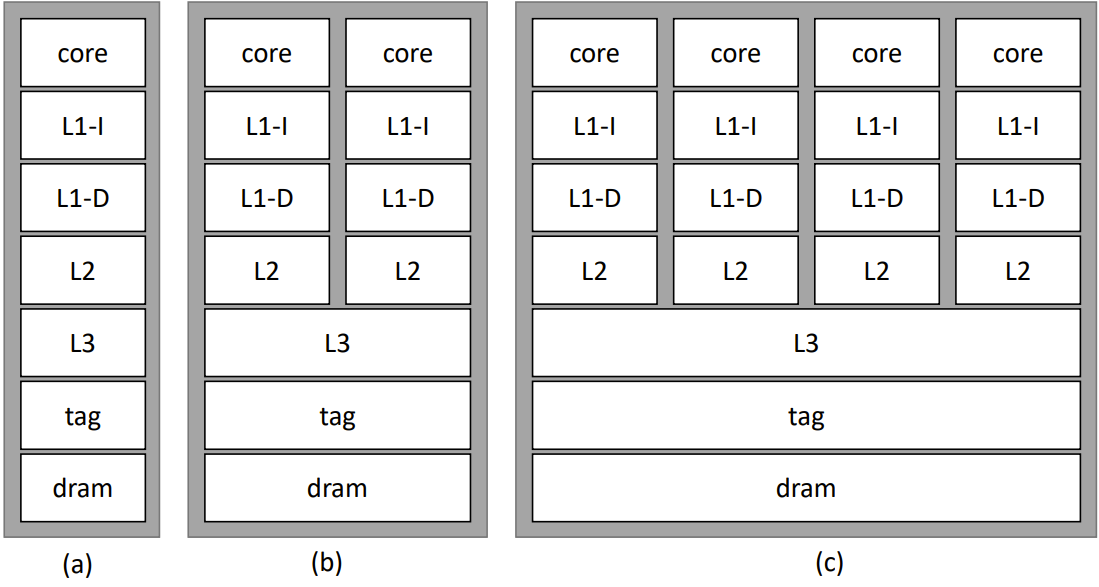
\includegraphics[width=0.7\textwidth]{cores.png}
        \caption{Experiment plan for 1, 2, and 4 core architectures.}
        \label{arch}
    \end{figure}

    \begin{figure}[htb!]
        \centering 
        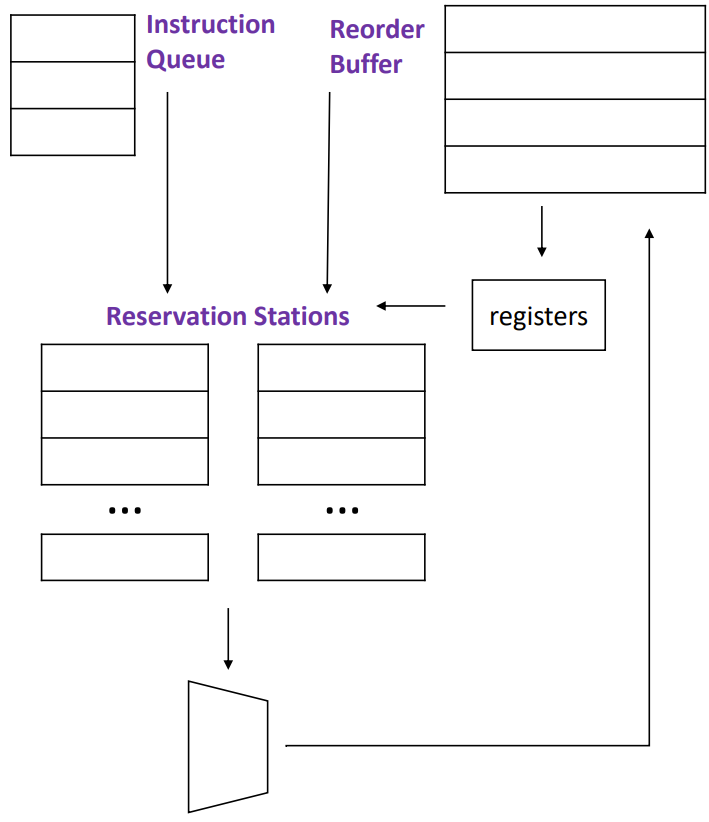
\includegraphics[width=0.5\textwidth]{rob.png}
        \caption{Experiment plan for reservation station entry sweep.}
        \label{rob}
    \end{figure}
    \clearpage

    \bibliographystyle{acm}%Used BibTeX style is acm
    \bibliography{sources}

\end{document}